% --- CHAPTER 7: OPERATIONAL HANDS-ON AND SECURITY VERIFICATION ---
\section{Beyond the User Guide: Operational Hands-On and Security Handshake Verification}
\label{sec:user_guide}

This chapter provides a comprehensive reference manual for the AdriaBOX Command-Line Interface (CLI) and documents the end-to-end operational verification performed on a live deployment. Rather than presenting abstract commands, this section describes a functional workflow mapping physical interactions to the automated test validations performed on the system architecture.

\subsection{The AdriaBOX CLI Reference Manual}
The client-side interface decouples core distributed protocols into human-friendly execution commands. Control operations rely on JSON payload metadata exchanges over HTTP REST, whereas data operations route raw payload byte chunks across isolated TCP streaming sockets. Table~\ref{tab:cli_manual} maps the complete, production-grade command matrix implemented inside the core routing controller.

\begin{table}[htbp]
\small
\centering
\caption{AdriaBOX CLI Reference Manual, Privileges, and Functional Syntax Mapping}
\label{tab:cli_manual}
\vspace{2mm}
\begin{tabularx}{\textwidth}{|l|c|X|p{6.2cm}|}
\hline
\textbf{Command} & \textbf{Privilege} & \textbf{Functional Description} & \textbf{Syntax Syntax and Example} \\ \hline
\texttt{register} & Tenant & Generates a new tenant profile. & \texttt{adria register <user> <psw>} \newline \textit{es. adria register sam 123} \\ \hline
\texttt{login} & Tenant & Requests a cryptographically signed JWT token. & \texttt{adria login <user> <psw>} \newline \textit{es. adria login sam 123} \\ \hline
\texttt{whoami} & Tenant & Displays token parameters and tenant roles. & \texttt{adria whoami} \newline \textit{es. adria whoami} \\ \hline
\texttt{logout} & Tenant & Discards the local storage session descriptor. & \texttt{adria logout} \newline \textit{es. adria logout} \\ \hline
\texttt{upload} & Tenant & Slices and replicates binary files into data nodes. & \texttt{adria upload <local\_path> [-d <rem\_dir>]} \newline \textit{es. adria upload file.zip -d /dir} \\ \hline
\texttt{download} & Tenant & Fetches chunks via pipeline synchronization. & \texttt{adria download <rem\_path> [-o <loc\_dest>]} \newline \textit{es. adria download /dir/file.zip} \\ \hline
\texttt{rm} & Tenant & Erases metadata entries and data plane segments. & \texttt{adria rm <rem\_filepath>} \newline \textit{es. adria rm /dir/file.zip} \\ \hline
\texttt{mkdir} & Tenant & Generates an isolated remote directory structure. & \texttt{adria mkdir <dir\_path>} \newline \textit{es. adria mkdir /backup} \\ \hline
\texttt{rmdir} & Tenant & Clears custom path structures recursively. & \texttt{adria rmdir <dir\_path>} \newline \textit{es. adria rmdir /backup} \\ \hline
\texttt{mv} & Tenant & Executes dynamic path shifts or entry renames. & \texttt{adria mv <source> <destination>} \newline \textit{es. adria mv /src.bin /dest.bin} \\ \hline
\texttt{quota} & Tenant & Displays real-time volumetric byte footprints. & \texttt{adria quota} \newline \textit{es. adria quota} \\ \hline
\texttt{cluster-status} & Admin & Queries active health metrics for the 12 nodes. & \texttt{adria cluster-status} \newline \textit{es. adria cluster-status} \\ \hline
\texttt{users} & Admin & Displays registered footprints across all tenants. & \texttt{adria users} \newline \textit{es. adria users} \\ \hline
\texttt{userdel} & Admin & Purges a tenant profile and scrubs database blocks. & \texttt{adria userdel <username>} \newline \textit{es. adria userdel sam} \\ \hline
\end{tabularx}
\end{table}

\subsection{Live Execution In Vivo Validation Spectrum}
To establish the practical resilience of the framework, this subsection chronicles a live multi-tenant execution cycle, focusing on chunk fragmentation, permission boundaries, error handling, and garbage collection. This empirical evaluation acts as a real-time sanity test designed to anchor the mass automated test cases developed within our validation suite.

\subsubsection{Tenant Onboarding and Volumetric Chunk Splitting Topology}
The operational verification begins with an unauthenticated workstation initializing an execution layout inside the isolated container \texttt{adriabox-client-max}. The operator generates a local test file containing exactly 512~MB of pseudo-random data (\texttt{512MB.zip}). 

A new user account named \texttt{max} is registered and logged in to establish an active JWT environment session wrapper. The initialization sequence is executed directly through the client-space shell as follows:

\begin{samepage}
\begin{verbatim}
root@989900287bec:/app# truncate -s 512M 512MB.zip
root@989900287bec:/app# poetry run adria register max 123
root@989900287bec:/app# poetry run adria login max 123
root@989900287bec:/app# poetry run adria mkdir /backup
root@989900287bec:/app# poetry run adria upload 512MB.zip -d /backup
\end{verbatim}
\end{samepage}

The execution of the chunk allocation routine triggers automated chunk division protocols. The system splits the 512~MB binary asset into exactly 8 uniform blocks weighing 64~MB ($67,108,864$~bytes) each, routing them sequentially to the cluster targets, as shown in Figure~\ref{fig:upload_live}.

\begin{figure}[htbp]
    \centering
    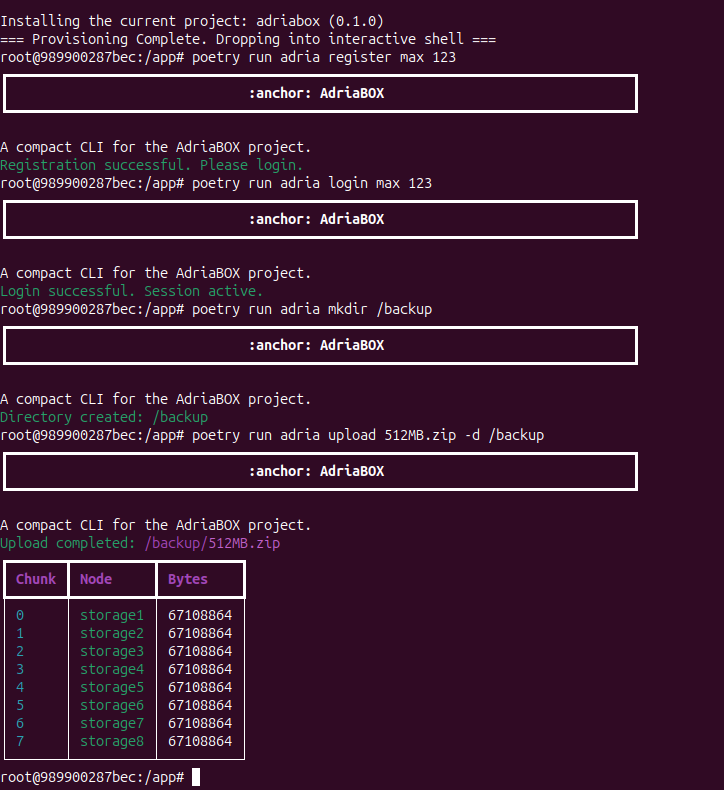
\includegraphics[width=0.85\textwidth]{images/7.1-screenshot.png}
    \caption{Live Console Log Output: User Onboarding, Isolated Path Registration, and 512~MB Volumetric Chunk-Splitting Execution.}
    \label{fig:upload_live}
\end{figure}

This mapping validates that data layout strategies process high-volume files without experiencing memory exhaustion leaks, allocating segments across distinct physical paths inside the containerized storage cluster.

\subsubsection{Mitigation of Information Leakage: Prevention of Resource Enumeration}
A critical security challenge in multi-tenant shared-storage structures involves avoiding information leakage across unlinked workspaces. If an attacker guesses a private directory path belonging to another tenant, an insecure control plane router might return a \texttt{403 Forbidden} error token. Although this token blocks data acquisition, it confirms the existence of the file, enabling resource mapping attacks.

To address this, the AdriaBOX backend forces an opaque security mapping paradigm via custom exception interceptors. To test this defense, a separate tenant named \texttt{sam} logs into their client container and attempts to access the data asset belonging to \texttt{max}:

\begin{samepage}
\begin{verbatim}
root@787b93b6137a:/app# poetry run adria login sam 123
root@787b93b6137a:/app# poetry run adria download /backup/512MB.zip
\end{verbatim}
\end{samepage}

As shown in Figure~\ref{fig:resource_enumeration}, the metadata tracking router intercepts the unauthorized identity claim and maps the security boundary to an uninformative, human-friendly error state.

\begin{figure}[htbp]
    \centering
    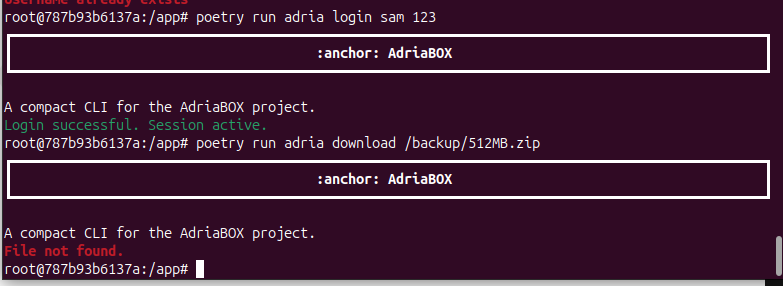
\includegraphics[width=0.85\textwidth]{images/7.2-screenshot.png}
    \caption{Live Security Verification: Mitigation of Information Leakage via Opaque Path Hiding Interception.}
    \label{fig:resource_enumeration}
\end{figure}

The system returns a generic \texttt{File not found.} notification, ensuring that private resources remain indistinguishable from non-existent data elements. Figure~\ref{fig:puml_exception} charts the architectural sequence of this defensive routine.

\begin{figure}[htbp]
    \centering
    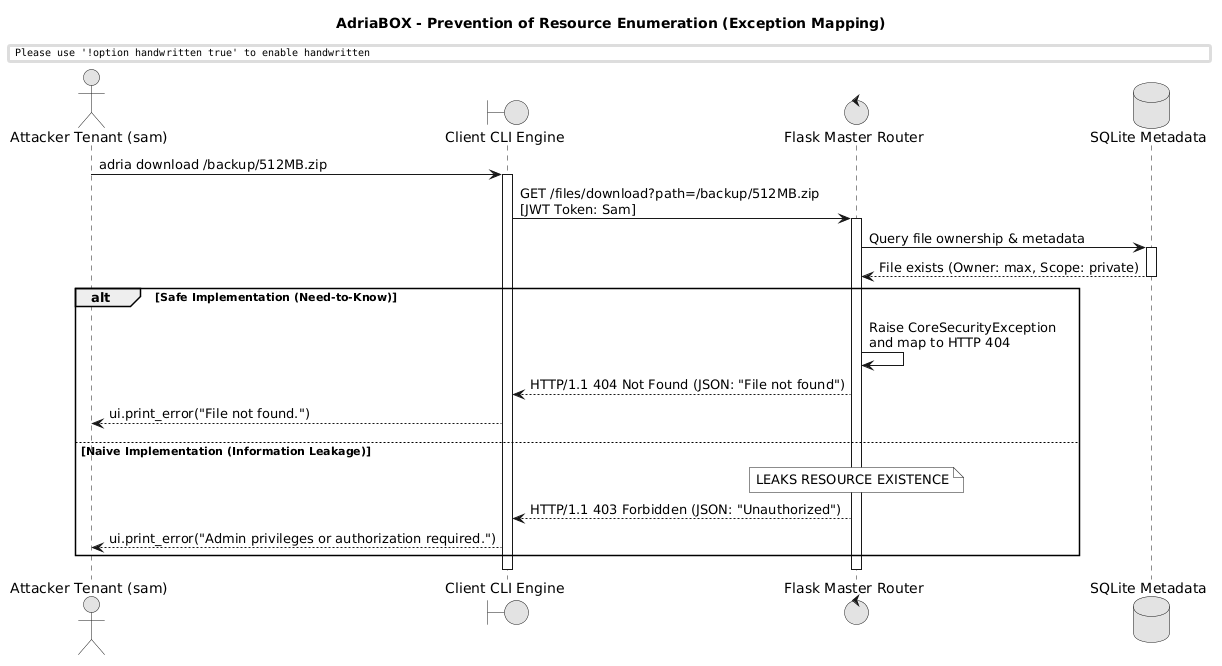
\includegraphics[width=0.95\textwidth]{plantuml/7.1-exception-mitigation.png}
    \caption{UML Sequence Diagram: Exception Mapping Protocol Enforcing Resource Enumeration Shielding.}
    \label{fig:puml_exception}
\end{figure}

\subsubsection{Client-Side Exception Parsing Asymmetry In Vivo Tracker}
While the protection matrix is applied uniformly on backend API endpoints, the live execution trace highlights an implementation asymmetry in the client-side parsing modules. 

When the tenant \texttt{sam} attempts to rename or move the private asset using the \texttt{mv} directive, the obfuscation routine responds with a secure HTTP 404 status. The command-line driver handles this response differently, bypasses clean formatting wrappers, and prints the raw network library traceback string on the screen:

\begin{samepage}
\begin{verbatim}
root@787b93b6137a:/app# poetry run adria mv /backup/512MB.zip /backup/hacked.zip
\end{verbatim}
\end{samepage}

Figure~\ref{fig:mv_asymmetry} captures this behavior on the terminal interface.

\begin{figure}[htbp]
    \centering
    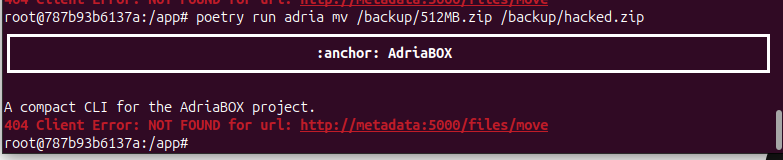
\includegraphics[width=0.85\textwidth]{images/7.3-pictures.png}
    \caption{Live Integration Traceback: Client-Side Exception Handling Asymmetry on Move Action.}
    \label{fig:mv_asymmetry}
\end{figure}

The raw output trace confirms that while backend security boundaries remain intact, the \texttt{mv} handler relies directly on the underlying library's status checker without intercepting the status code, showing a clear area for further interface formatting refinements.

\subsubsection{Administrative Ownership Audit and Cluster Footprint Tracking}
Administrative tasks are validated using the privileged identity token \texttt{devil}, following out-of-band role elevation directly on the SQLite database. This profile bypasses tenancy visibility bounds to audit cluster resource allocation. 

The administrator invokes the global directory analyzer inside their client shell to inspect the membership index and verify active node status parameters:

\begin{samepage}
\begin{verbatim}
root@1deca995ffc8:/app# poetry run adria login devil 666
root@1deca995ffc8:/app# poetry run adria users
root@1deca995ffc8:/app# poetry run adria cluster-status
\end{verbatim}
\end{samepage}

The live administrative status table returned by the server is shown in Figure~\ref{fig:admin_list}.

\begin{figure}[htbp]
    \centering
    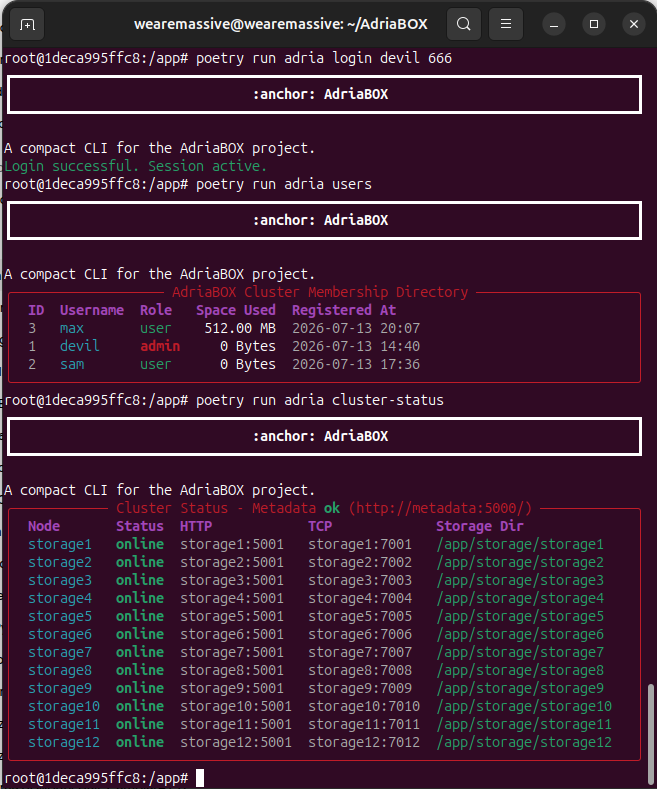
\includegraphics[width=0.85\textwidth]{images/7.4-Screenshot.png}
    \caption{Live Administrative Panel View: Membership Footprint Directory and Storage Cluster Telemetry.}
    \label{fig:admin_list}
\end{figure}

The table reports an exact log footprint allocation of 512.00~MB for user \texttt{max}, while the status table confirms that all 12 storage nodes are currently running online. This confirms that the control plane records metrics based on the logical size of user files, decoupling accounting tasks from backend storage replication layers.

\subsubsection{Privileged Profile Purging and Asynchronous Asset Reclamation}
The operational lifecycle concludes with the automated destruction of user data assets. When an account is removed via administrative authority, the master system must scrub all corresponding metadata records and execute an asynchronous garbage collection sequence across the 12 data nodes to reclaim storage capacity. 

The administrator invokes the structural purge command:

\begin{samepage}
\begin{verbatim}
root@1deca995ffc8:/app# poetry run adria userdel max
root@1deca995ffc8:/app# poetry run adria users
\end{verbatim}
\end{samepage}

Figure~\ref{fig:purge_live} details the console status following this administrative action.

\begin{figure}[htbp]
    \centering
    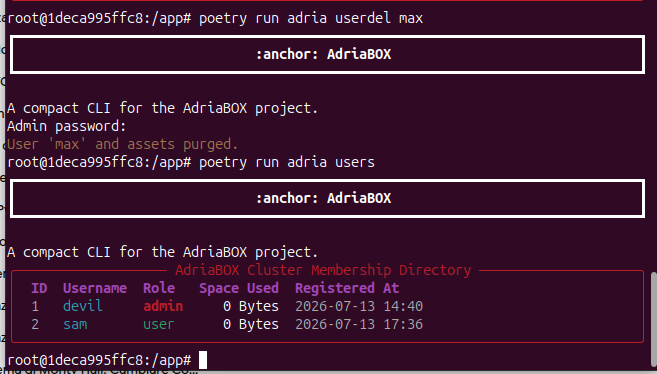
\includegraphics[width=0.85\textwidth]{images/7.5-Screenshot.png}
    \caption{Live Administrative Garbage Collection: Synchronous Account Purge and Data Block Reclamation.}
    \label{fig:purge_live}
\end{figure}

The confirmation message verifies that the database fields have been successfully removed and the space used is reset to zero, returning the cluster to a balanced state.
